%! TeX program = lualatex
\documentclass[12pt,a4paper]{article}

\usepackage[nil]{babel}
\usepackage{unicode-math}
\usepackage[svgnames]{xcolor}
\usepackage{lmodern}
\usepackage{graphicx}
\usepackage{wrapfig}
\usepackage{float}
\usepackage{parskip}

\babelprovide[import=el, main, onchar=ids fonts]{greek} % can also do import=el-polyton
\babelprovide[import, onchar=ids fonts]{english}

\babelfont{rm}
          [Language=Default]{Liberation Sans}
\babelfont[english]{rm}
          [Language=Default]{Liberation Sans}
\babelfont{sf}
          [Language=Default]{Liberation Sans}
\babelfont{tt}
          [Language=Default]{Liberation Sans}

%Enter Title Here
 \title{Sequence-diagrams-v0.1 \\ LibShare}
\author{\textbf{Ονόματα / ΑΜ / Έτος:} \\ Γρηγόρης Καπαδούκας / 1072484 / 4\textdegree \\ Χρήστος Μπεστητζάνος / 1072615 / 4\textdegree \\ Νικόλαος Αυγέρης / 1067508 / 5\textdegree \\ Περικλής Κοροντζής / 1072563 / 4\textdegree}

\begin{document}

\makeatletter
\begin{center}
	\LARGE{\@title} \\
	\pagebreak
    \begin{LARGE}\@author\end{LARGE}
    \pagebreak
\end{center}

%Insert Body Here
\section{Sequence Diagrams}

\subsection{Αναζήτηση βιβλίων / χρήστη / αιτήσεων}
\begin{figure}[H]
	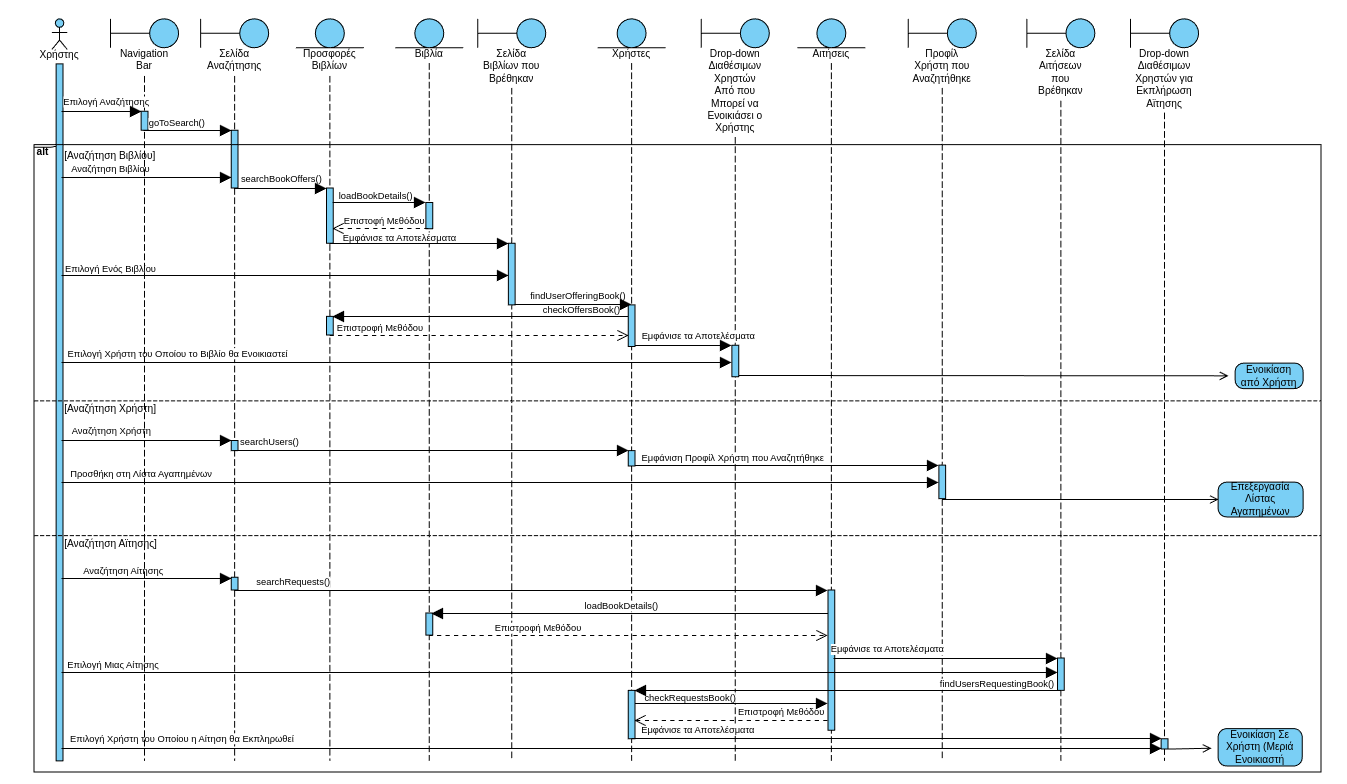
\includegraphics[width=\textwidth]{Search Sequence.png}
	\caption{Sequence Diagram: Αναζήτηση βιβλίων / χρήστη / αιτήσεων}
	\label{Sequence Diagram: Αναζήτηση βιβλίων / χρήστη / αιτήσεων}
\end{figure}

\subsection{Αποδοχή Προσφοράς Βιβλίου και Ενοικίαση}
\begin{figure}[H]
	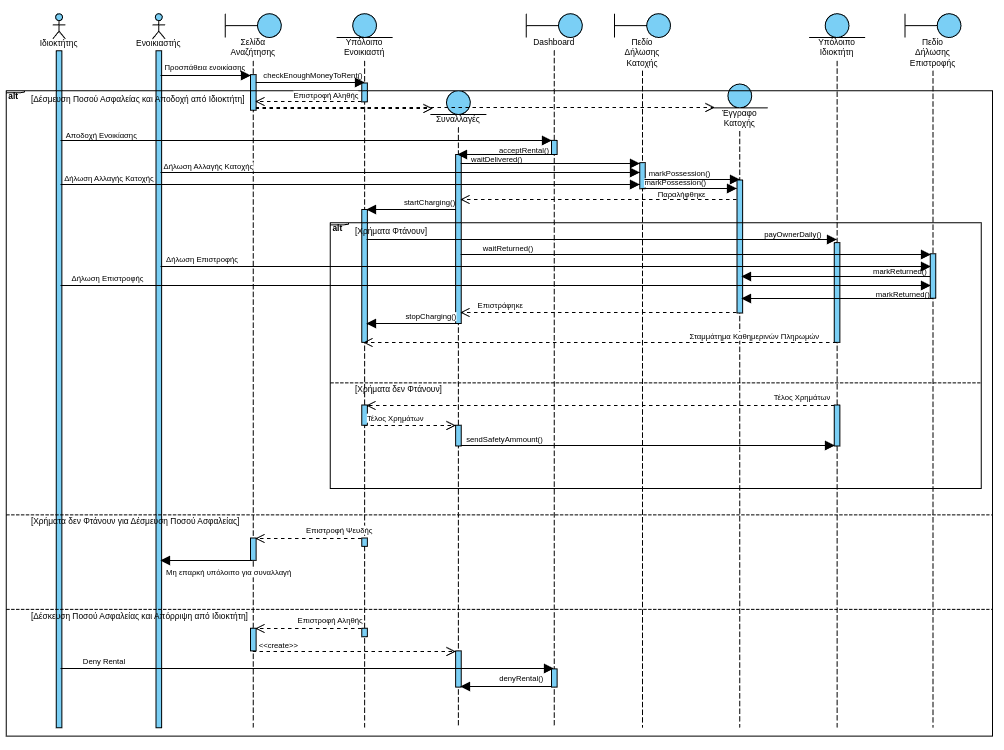
\includegraphics[width=\textwidth]{Accept Book Offer and Rent Sequence.png}
	\caption{Sequence Diagram: Αποδοχή Προσφοράς Βιβλίου και Ενοικίαση}
	\label{Sequence Diagram: Αποδοχή Προσφοράς Βιβλίου και Ενοικίαση}
\end{figure}

\subsection{Αποδοχή Αίτησης Βιβλίου και Ενοικίαση}
\begin{figure}[H]
	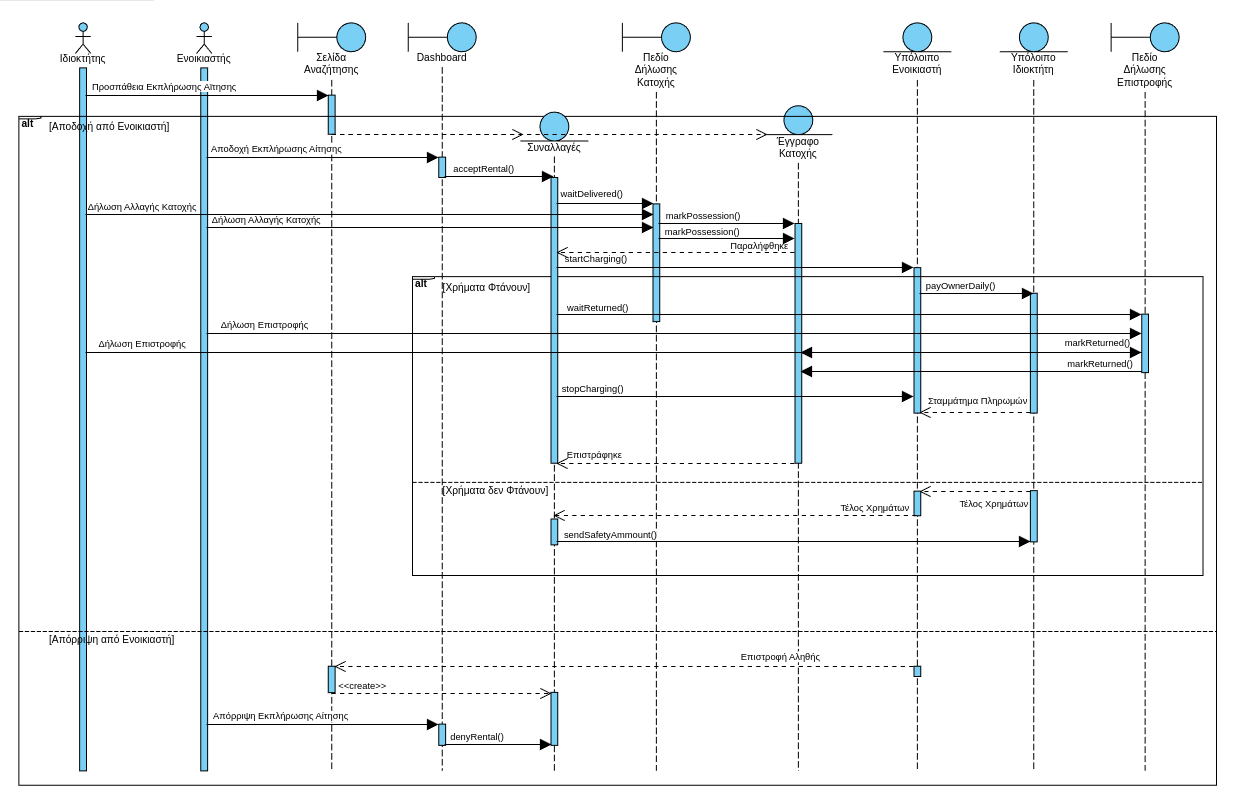
\includegraphics[width=\textwidth]{Accept Request Offer and Rent Sequence.png}
	\caption{Sequence Diagram: Αποδοχή Αίτησης Βιβλίου και Ενοικίαση}
	\label{Sequence Diagram: Αποδοχή Αίτησης Βιβλίου και Ενοικίαση}
\end{figure}

\subsection{Διαχείριση των βιβλίων που προσφέρει ο χρήστης προς ενοικίαση από άλλους}
\begin{figure}[H]
	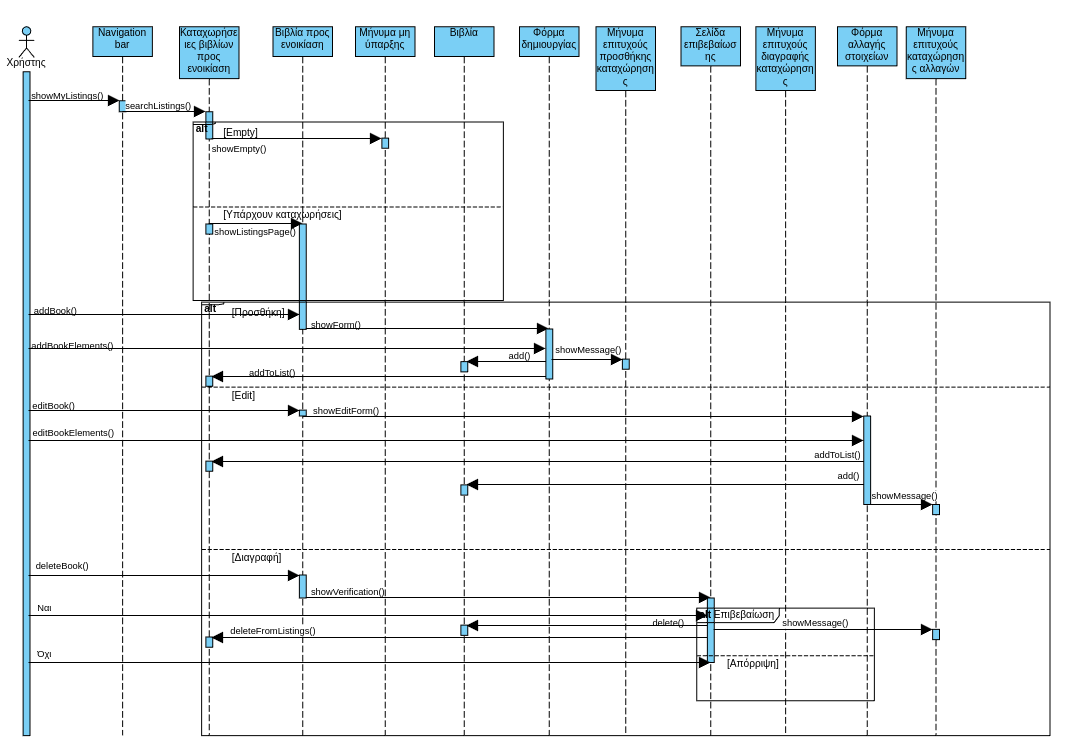
\includegraphics[width=\textwidth]{Manage User Book Listings Sequence.png}
	\caption{Sequence Diagram: Διαχείριση των βιβλίων που προσφέρει ο χρήστης προς ενοικίαση από άλλους}
	\label{Sequence Diagram: Διαχείριση των βιβλίων που προσφέρει ο χρήστης προς ενοικίαση από άλλους}
\end{figure}

\subsection{Διαχείριση των αιτήσεων που έχει κάνει ο χρήστης}
\textbf{Σημείωση:} Στο διάγραμμα αυτό τα εναλλακτικά blocks μέσα στο εναλλακτικό block "Προσθήκη σε empty" και "Προσθήκη με ήδη υπάρχουσα" είναι τα ίδια, απλά στη πρώτη περίπτωση λόγω περιορισμού χώρου δεν είναι τόσο ευκρινής το διάγραμμα.
\begin{figure}[H]
	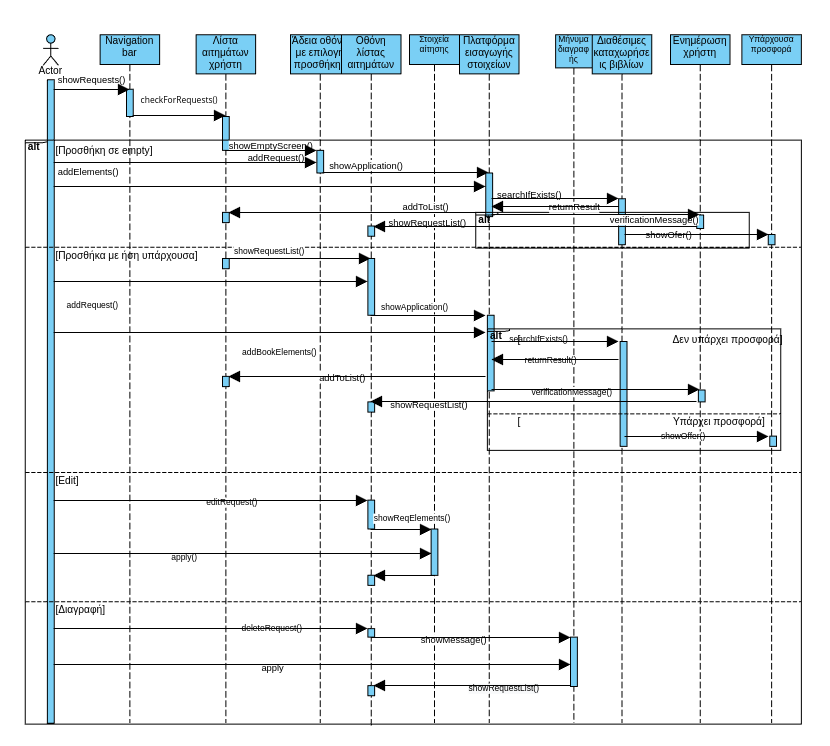
\includegraphics[width=\textwidth]{Manage User Requests Sequence.png}
	\caption{Sequence Diagram: Διαχείριση των αιτήσεων που έχει κάνει ο χρήστης}
	\label{Sequence Diagram: Διαχείριση των αιτήσεων που έχει κάνει ο χρήστης}
\end{figure}

\subsection{Αξιολόγηση άλλων χρηστών μετά από την ολοκλήρωση συναλλαγής}
\begin{figure}[H]
	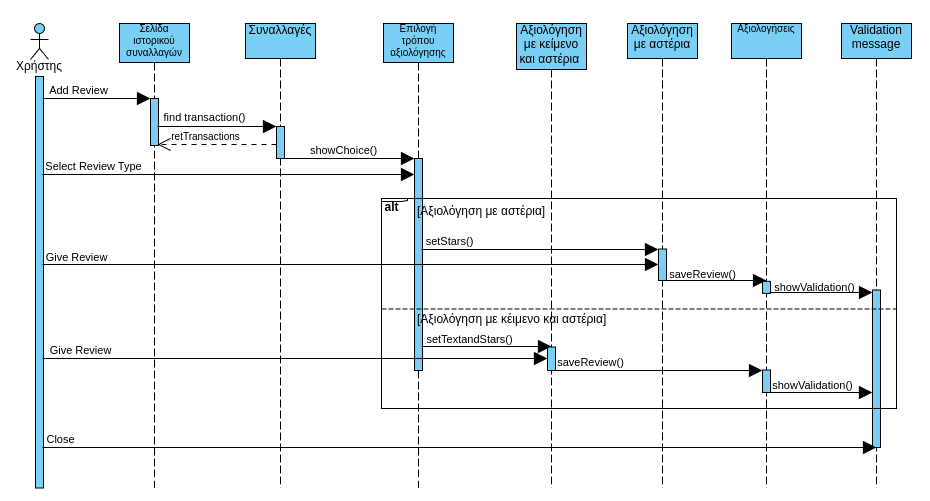
\includegraphics[width=\textwidth]{Review after Transaction Sequence.png}
	\caption{Sequence Diagram: Αξιολόγηση άλλων χρηστών μετά από την ολοκλήρωση συναλλαγής}
	\label{Sequence Diagram: Αξιολόγηση άλλων χρηστών μετά από την ολοκλήρωση συναλλαγής}
\end{figure}


\subsection{Προβολή και Επεξεργασία στοιχείων λογαριασμού χρήστη}
\begin{figure}[H]
	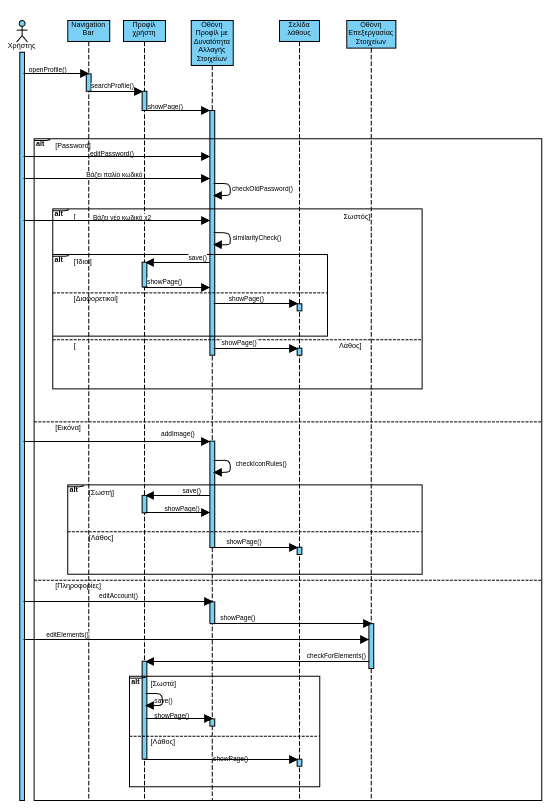
\includegraphics[width=\textwidth]{View and Edit User Account Details Sequence.png}
	\caption{Sequence Diagram: Προβολή και Επεξεργασία στοιχείων λογαριασμού χρήστη}
	\label{Sequence Diagram: Προβολή και Επεξεργασία στοιχείων λογαριασμού χρήστη}
\end{figure}

\subsection{Επεξεργασία χρηματικού υπολοίπου χρήστη}
\begin{figure}[H]
	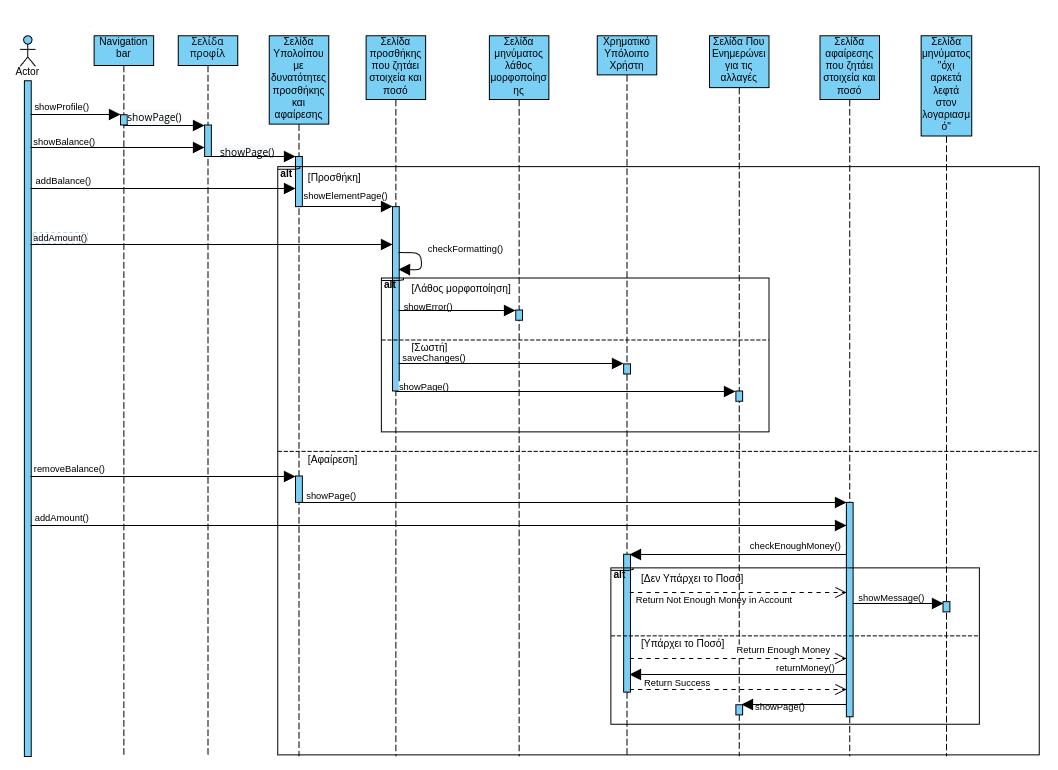
\includegraphics[width=\textwidth]{Edit User Balance Sequence.png}
	\caption{Sequence Diagram: Επεξεργασία χρηματικού υπολοίπου χρήστη}
	\label{Sequence Diagram: Επεξεργασία χρηματικού υπολοίπου χρήστη}
\end{figure}

\subsection{Επεξεργασία λίστας αγαπημένων και χρήση συστήματος ειδοποιήσεων}
\begin{figure}[H]
	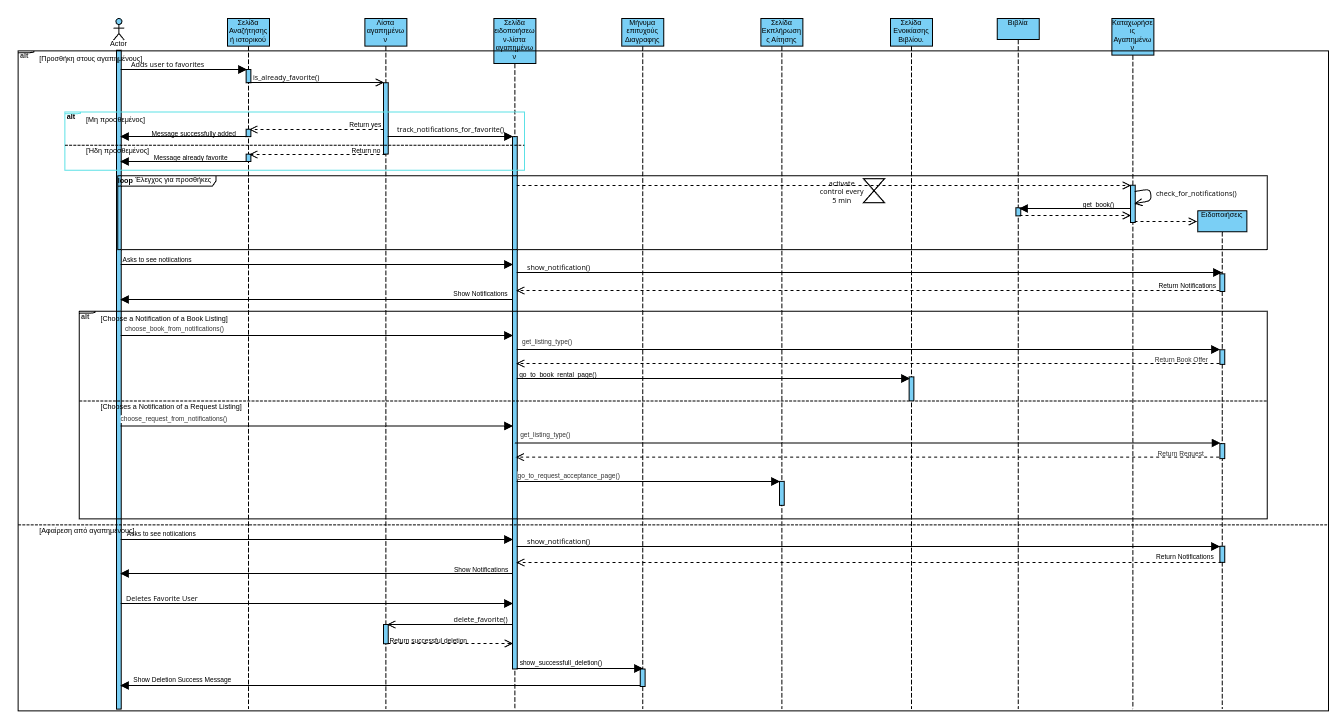
\includegraphics[width=\textwidth]{Favorite Users and Notification System Sequence.png}
	\caption{Sequence Diagram: Επεξεργασία λίστας αγαπημένων και χρήση συστήματος ειδοποιήσεων}
	\label{Sequence Diagram: Επεξεργασία λίστας αγαπημένων και χρήση συστήματος ειδοποιήσεων}
\end{figure}

\subsection{Προβολή ιστορικού συναλλαγών και στατιστικών}
\begin{figure}[H]
	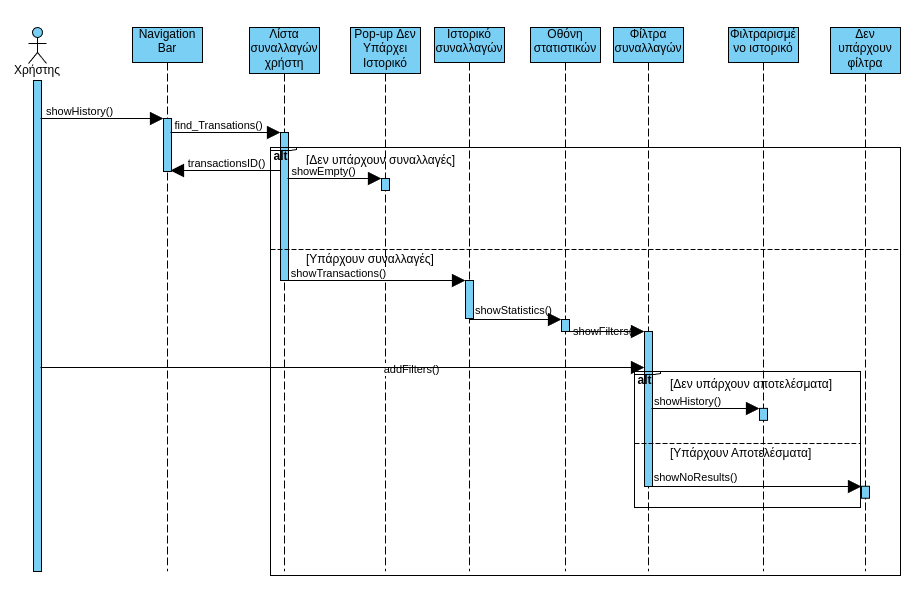
\includegraphics[width=\textwidth]{History and Statistics Sequence.png}
	\caption{Sequence Diagram: Προβολή ιστορικού συναλλαγών και στατιστικών}
	\label{Sequence Diagram: Προβολή ιστορικού συναλλαγών και στατιστικών}
\end{figure}

\section{Συμμετοχή και Ρόλοι στη Συγγραφή του Κειμένου}
\begin{enumerate}
	\item \textbf{Γρηγόρης Καπαδούκας:} Author (Κεφαλαίων 1.1, 1.2, 1.3), Editor (Κεφαλαίων 1.9), Reviewer Όλων
	\item \textbf{Χρήστος Μπεστητζάνος:} Author (Κεφαλαίων 1.5, 1.6), Editor (Κεφαλαίων 1.4, 1.7, 1.8, 1.10), Reviewer Όλων
   	\item \textbf{Νικόλαος Αυγέρης:} Author (Κεφαλαίων 1.7, 1.8, 1.9)
	\item \textbf{Περικλής Κοροντζής:} Author (Κεφαλαίων 1.4, 1.10)
\end{enumerate}

\end{document}
